\subsection{Encryption}

(Rationale for choosing pub-key encryption?)

\subsubsection{Key Generation}

"An elliptic curve key pair is associated with a particular set of domain parameters": (Hankerson p. 180)

\( D = (q,FR,a,b,P,n,h) \)

Where \(q\) is the field order, \(FR\) is the field representation used for the elements of \( \mathbb{ F }_q \),
\(a, b\) the coefficients that define the equation of the curve (Weierstrass form), \(P\) a point on the curve which
has \emph{prime order} (??), \(n\) the order of \(P\), \(h = \#E(\mathbb{F}_q) / n\) the cofactor. (Note: Left out:
\(S\), the seed for randomly generated curves) (Hankerson et.al. p. 172)

(Note: Hankerson et.al. p. 173 about validation of domain parameters?)

"The public key is a randomly selected point \(Q\) in the group \( \langle P \rangle \) generated by \(P\). The corresponding
private key is \(d = log_p Q\)." \(Q\) is computed as \(Q = dP\). Computing \(d\) from \(Q\) is "precisely the elliptic curve
discrete logarithm problem". (Hankerson et.al. p. 180)

(Note: Hankerson et.al. pp. 180-181 about public key validation - proving that a private key exists, without finding it. Something
should be added about this, although maybe not until the implementation part? It is less important to the structure of the program.
It should be noted that \emph{h} in our case is probably 1, which may make some things easier...)

A key generation algorithm takes the Domain Parameters as input and generates the key pair. (Hankerson et.al. p. 188)

\subsubsection{Public-Key Encryption}

ECIES, The Elliptic Curve Integrated Encryption Scheme, is a variant of the ElGamal public-key encryption scheme. This scheme relies
on a key derivation function, a symmetric encryption scheme, such as AES, which will be used in the naive implementation, and a
message authentication code (MAC) algorithm, such as HMAC. (Hankerson et.al. p. 189)

\begin{figure}[ht!]
	\centering
	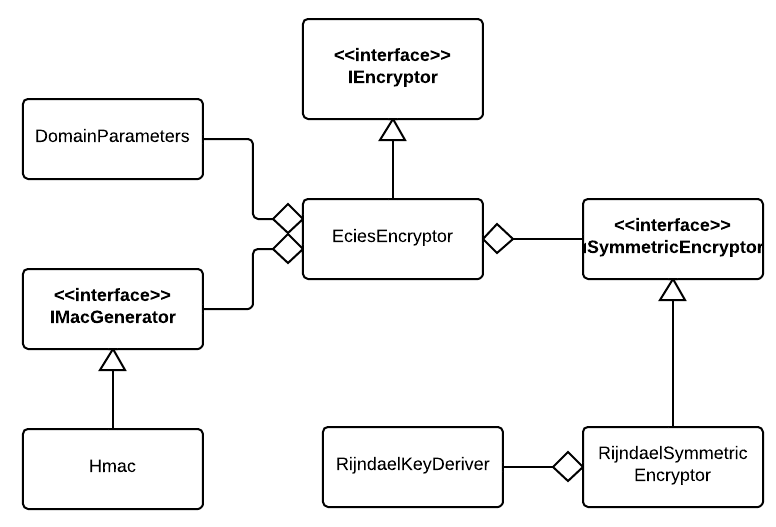
\includegraphics[width=90mm]{img/naive_implementation__encryption__ecies_class_diagram.png}
	\caption{Class Diagram of structure around the ECIES encryption implementation}
	\label{ecies_class_diagram}
\end{figure}

This adds new dependencies to the project: AES and HMAC.

C\# has built-in support for Rijndael\footnote{http://msdn.microsoft.com/en-us/library/system.security.cryptography.rijndaelmanaged.aspx}
(AES), and trusting this implementation is assumed safe for the scope of this project. Again, the importance of the naive implementation
is to show a full, working stack with naive implementations of the basics of Elliptic Curves (but not other basic constructs).

It is possible to set a specific key in \verb+RijndaelManaged+, so what is now needed is the key derivation function, which will have to
be constructed for the purpose.

--- key deriv func ---

HMAC is supported in C\# as well\footnote{http://msdn.microsoft.com/en-us/library/system.security.cryptography.hmac.aspx}.

--- actual encryption ---